%%%% Proceedings format for most of ACM conferences (with the exceptions listed below) and all ICPS volumes.
\documentclass[sigconf]{acmart}
%%%% As of March 2017, [siggraph] is no longer used. Please use sigconf (above) for SIGGRAPH conferences.

%%%% Proceedings format for SIGPLAN conferences 
% \documentclass[sigplan, anonymous, review]{acmart}

%%%% Proceedings format for SIGCHI conferences
% \documentclass[sigchi, review]{acmart}

%%%% To use the SIGCHI extended abstract template, please visit
% https://www.overleaf.com/read/zzzfqvkmrfzn

\usepackage{float}
\usepackage{booktabs} % For formal tables


% Copyright
%\setcopyright{none}
%\setcopyright{acmcopyright}
%\setcopyright{acmlicensed}
\setcopyright{rightsretained}
%\setcopyright{usgov}
%\setcopyright{usgovmixed}
%\setcopyright{cagov}
%\setcopyright{cagovmixed}


% DOI
\acmDOI{10.475/123_4}

% ISBN
\acmISBN{123-4567-24-567/08/06}

%Conference
\acmConference[WOODSTOCK'97]{ACM Woodstock conference}{July 1997}{El
  Paso, Texas USA} 
\acmYear{1997}
\copyrightyear{2016}


\acmArticle{4}
\acmPrice{15.00}

% These commands are optional
%\acmBooktitle{Transactions of the ACM Woodstock conference}
\editor{Jennifer B. Sartor}
\editor{Theo D'Hondt}
\editor{Wolfgang De Meuter}

\begin{document}
\title{An Analysis of Indexing and Querying Strategies on Technologically Assisted Review Tasks}
%\titlenote{Produces the permission block, and copyright information}
% \subtitle{Extended Abstract}
% \subtitlenote{The full version of the author's guide is available as \texttt{acmart.pdf} document}


\author{Author 1}
\affiliation{%
  \institution{institution}
  \city{city} 
  \state{state} 
}

\author{Author 2}
\affiliation{%
  \institution{institution}
  \city{city} 
  \state{state}
}

\author{Author 3}
\affiliation{%
  \institution{institution}
  \city{city} 
  \country{country}}

% The default list of authors is too long for headers.
\renewcommand{\shortauthors}{B. Trovato et al.}

\begin{abstract}

This paper is a preliminary experimentation study using the CLEF collection for evaluating the effectiveness of different indexing methodologies of documents and query parsing techniques. Furthermore, it is an attempt to advance and share the efforts of observing the characteristics and helpfulness of various methodologies for indexing PubMed documents and for different topic parsing techniques to produce queries. For this purpose, our research included experimentation with different document indexing methodologies, by utilising existing tools, such as the Lucene4IR\footnote{https://github.com/lucene4ir} (L4IR) information retrieval (IR) system, the Technology Assisted Reviews (TAR) for Empirical Medicine tool\footnote{https://github.com/CLEF-TAR/tar} for parsing topics of the CLEF collection and the TREC evaluation tool\footnote{http://trec.nist.gov/trec\_eval} to appraise system's performance.  

\end{abstract}

%
% The code below should be generated by the tool at
% http://dl.acm.org/ccs.cfm
% Please copy and paste the code instead of the example below. 
%
\begin{CCSXML}
<ccs2012>
 <concept>
  <concept_id>10002951.10003317.10003359</concept_id>
  <concept_desc> Information systems~Evaluation</concept_desc>
  <concept_significance>500</concept_significance>
 </concept>
 </ccs2012>  
\end{CCSXML}

\ccsdesc[500]{Information systems~Evaluation of retrieval results}


\keywords{PubMed, Medical Information Retrieval (IR), Indexing Schemata, Measurement, Performance, Query Parser, CLEF Collection, BM25}


\maketitle

\section{Introduction}

The recently entrenched CLEF 2017 eHealth Task 2 required from the participants to rank a set of PubMed abstracts (A) given the results retrieved from the previous Task 1. The track had 2 objectives. Create an effective ranking of the documents, such that all of the relevant abstracts are recovered as soon as possible and determine a subgroup of (A), which contains as many of the relevant abstracts for the least effort (Kanoulas et al., 2017) \cite{kanoulas2017clef}. The participants were given the associated qrels judgments file, which follows the TREC format Topic number, Iteration, PubMed identification number, Relevancy, a binary code of 0 (not relevant) and 1 (relevant). The order of documents in the qrels file does not suggest degree of relevance. Documents not occurring in the qrels file were not judged by the human assessor and are presumed to be irrelevant in the evaluations. A more detailed description of the task can be found here\footnote{://sites.google.com/site/clefehealth2017/task-2}.
%======================================================
It is important to note some of the different approaches in the submissions of the participants. For example Alharbi et al. \cite{alharbiranking} utilised the review title and Boolean query to order the abstracts retrieved by the query, by applying standard similarity measures. According to the authors \cite{alharbiranking} the title and terms extracted from the Boolean query contributed the most useful information for this task. Their methodology made use of 3 topic parts, the text of the title, the terms and Mesh items parsed from the Boolean query. The Mesh items were preprocessed with the same approach applied on the Boolean query. Moreover, preprocessing was added to the PubMed abstracts and data extracted from the topics. The text was tokenised, changed to lower case, stop words were taken out and the rest of the tokens were stemmed. Lastly, the data extracted from the topic and every abstract was converted into TF-IDF weighted vectors \cite{alharbiranking} to calculate similarity among the topic and every abstract using the cosine metric for the pair of vectors.
%======================================================
Ecnu et al. \cite{chen2017ecnu} used a customised Learning-to-Rank (L2R) model and the word2vec to represent queries and documents and compute their similarities by cosine distance. Their L2R model consists of 3 points, query expansion, feature extraction and model training. In the query expansion stage, they improved retrieval precision by expanding queries. 
In the feature extraction stage, they extracted features of each query document pair. When a document was retrieved under a query, it was connected with a weighting score and rank. Finally, in the learning phase of the L2R model, the relevance of a query-document pair was assessed with the random forest classifier.
%======================================================
Norman et al. used a system that builds on logistic regression \cite{norman122017limsi}, and implemented strategies to handle class imbalance and perform relevance feedback. Additionally,they tested 2 classifiers, logistic regression with stochastic gradient descent learning on the entire data and standard logistic regression trained using conventional methods on a subgroup of the data with added preprocessing to enhance the yield.
%======================================================
Nunzio et al. \cite{nunzio2017interactive} concentrated their work on discovering the optimal combination of certain hyper-parameters by utilising the training data available and a force brute strategy. This strategy created different query features of the identical information need given a minimum amount of relevance feedback. Furthermore, they decided to use a plain BM25 retrieval model and acquire the relevance feedback for the first abstract in the ranking list for each topic. Afterwards, they asked 2 different people to build 2 different queries according to the value of the feedback. The 2 queries are combined with the original one in different ways. Finally, they designed alternative strategies that use the following parameters, number of documents to assess in batches or iteratively, percent of documents to assess, maximum number of documents to assess per iteration, number of terms to add at each feedback iteration for the cost-effective evaluation and the minimum precision the system can reach before terminating the search.
%======================================================
Singh et al. utilised Lucene's inverted index to index the retrieved articles retrieved from PubMed query performed during a systematic review \cite{singhiiit}.
The query is processed for term boosting, fuzzy search and used for scoring documents according to TF-IDF similarity. Relevance feedback is used to update the query and become more pragmatic.
%======================================================
Essentially, different people have implemented different strategies and they all used different methods, so it is hard to determine what indexing strategy or querying parsing technique is best to perform for the initial round of retrieval.
%======================================================
\section{Research Questions}

Therefore, the following research questions, are raised: 
\begin{enumerate}
  \item[\textbf{RQ1}]  How do different indexing schemata affect performance? 
  \item[\textbf{RQ2}] How does the initial query extracted from the CLEF Topic affects performance?
\end{enumerate}

\section{Method}

\subsection{Data and Materials}

The data that was used is the CLEF collection\footnote{http://www.clef-initiative.eu/dataset/test-collection}. The complete CLEF collection consists of 198,365 XML documents, it contains 50 topics, a total of 266,967 abstracts and the number of relevant documents is  . Furthermore, each PubMed article set has a basic structure, that contains a PubMed article. The PubMed article consists of the Medline citation fields and the PubMed data and metadata fields. The Medline citation includes fields such as the ID of the PubMed document, date of creation and completion, ISO abbreviations, title and abstract of the article, the list of author(s), the MeSH heading list, the list of chemicals other information of the Medline Journal. The PubMed data contain information such as historical dates, the publication status and more information. Each topic of the CLEF collection contains the topic-ID, the title of the review and the Boolean query manually drafted and constructed by Cochrane experts and the collection of PubMed document identifiers (PMID) retrieved by executing the query in MEDLINE databases. For all of our indexes we used the standard tokeniser in L4IR, and a variety of token filters. The token filters used are the following: stopping, porter stemmer, generation of word parts, pattern replacement, lowercase and word delimiter with the key parameter of this token filter set to 'preserveOriginal'. Additionally, we utilised the L4IR (Azzopardi et al., 2017) \cite{azzopardi2017lucene4ir}, which consists a collaborative effort of researchers to extend the Lucene library and produce a group of statistical evaluation tools for common IR methods such as indexing and retrieval for different types of test collections. The L4IR, includes among other functions, 3 main applications: the IndexerApp, the RetrievalApp and the ExampleStatsApp. The IndexerApp, allows to index multiple different TREC collections, such as the Aquaint Collection, but also the PubMed collection. The RetrievalApp, is a batch retrieval application, which contains various retrieval algorithms, for example the BM25, the PL2 and more. Both the IndexerApp and the RetrievalApp applications can be configured appropriately by editing their parameters files 'index\_params.xml' and 'retrieval\_params.xml'. Finally, the ExampleStatsApp, is an application, which shows an example of accessing different metrics, such as term posting list, term positions, and more regarding the terms, the documents and the corpus. For the purposes of this study, we used the baseline retrieval algorithm used at CLEF 2017, BM25, to rank the document sets. Moreover, we utilised the CLEF TAR tool, for extracting parts from the topics of the CLEF collection, such as the ID, title and query of the topic and more. Additionally, we used Jupyter-Notebooks to automate the process of running experiments, but also to facilitate more testing in the future, in a larger experimentation setup (e.g. the incorporation of a greater number of indexing methodologies and query parsing techniques).

\subsubsection{Measures} \label{Measures}

The measurements we used for the purpose of this research are Mean Average Precision (MAP) (Table 1), Precision after 10, 20 and 30 documents (Table 2) and Interpolated Recall - Precision Averages (IRPA) at 0.10, 0.20 and 0.30 recall (Table 3).

\subsubsection{Indexing Schemata}

In our research we used 5 different indexing schemata, which are outlined below. Each indexing schema consists of a unique combination of XML fields. 

\begin{list}{$\square$}{\leftmargin=1em \itemindent=0em}
	\item[\textbf{1}] The  $1^{st}$ indexing schema indexed the Title, Abstract and PMID and was named 'TAP'.
    \item[\textbf{2}] The $2^{nd}$ indexing schema included the fields of the $1^{st}$ indexing schema along with the Author(s), the Journal title and the Year and was named '1+AJY'.
    \item[\textbf{3}] The $3^{rd}$ schema combined the XML fields of the $2^{nd}$ indexing schema with the Mesh Heading List (MHL) and was named '2+MHL'.
    \item[\textbf{4}] The $4^{th}$ indexing schema included the $2^{nd}$ indexing schema and the MedlineTA (MTA) field and was named '2+MTA'.
    \item[\textbf{5}] The $5^{th}$ indexing schema combined the  $2^{nd}$ indexing schema with the Mesh HL and the MedlineTA and was named '2+MHLMTA'.
\end{list}
%=================================================
\vspace{-0.2cm}

\subsection{Query Parser}

Furthermore, 3 different query parsers were implemented, so that the performance of the IR system L4IR could be tested by using different query variations. The 3 different query parsers that were used are listed below: 

\begin{list}{$\square$}{\leftmargin=1em \itemindent=0em}
	\item[\textbf{A}] The Title of the topic and was named 'title'.
    \item[\textbf{B}] The Query of the topic and was named 'query'.
    \item[\textbf{C}] The combination of the Title and Query of the topic and was named 'title and query'.
\end{list}

\section{Token Filter Pipeline}

\subsection{Retrieval Model and Parameters}

As mentioned above the IR model used was the BM25 and its free parameters b and $k_1$ were set to be 0.75 and 1.2 respectively, for this experimentation round. To compare our results, we used the SPSS statistical tool and the one-way ANOVA and one-way repeated measures ANOVA statistical test procedures. We denoted statistical significance at 5\%. The results from both statistical tests indicated significance at $p < 0.05$ and the $p-value < 0.00001$. More specifically, the one-way ANOVA and one-way repeated measures ANOVA procedures returned a total standard deviation of 0.0362, the F-ratio values were estimated at 233.5 and 1373.005 respectively and the total mean values were 0.0888 and 0.089 accordingly.

\section{Results}

\subsection{Tables}

% In the tables below we have captured the measurements \ref{Measures} of our retrieved results from L4IR using the trec\_eval tool. 
%=======================================================
\vspace{-0.25cm}
\begin{table}[h!]
\caption{Comparison of MAP between the 5 different indexing schemes and the 3 different query parsers}
\vspace{-0.1cm}
\centering
	\begin{tabular}{cccccc} 
\hline 
                & TAP & 1+AJY & 2+MHL & 2+MTA & 2+MHLMTA \\ \hline
title           & 0.1211     & 0.1237     & 0.135      & 0.1233     & 0.136      \\
query           & 0.039      & 0.0419     & 0.048      & 0.0419     & 0.0485     \\
title and query & 0.0836     & 0.0954     & 0.0993     & 0.0942     & 0.1013     \\ \hline
     \end{tabular}
\end{table}
\vspace{-0.6cm}
%=======================================================
\begin{table}[h!]
\centering
\caption{Comparison of precision after certain \# documents are retrieved  between the 5 different indexing schemes and the 3 different query parsers}
\vspace{-0.1cm}
\label{my-label}
\begin{tabular}{cccccc}
\hline
                & TAP & 1+AJY & 2+MHL & 2+MTA & 2+MHLMTA \\ \hline
\multicolumn{6}{r}{Precision after 10 documents retrieved}                       \\ \hline
title           & 0.258      & 0.29       & 0.274      & 0.29       & 0.284      \\
query           & 0.156      & 0.13       & 0.138      & 0.128      & 0.144      \\
title and query & 0.218      & 0.198      & 0.22       & 0.204      & 0.216      \\ \hline
\multicolumn{6}{r}{Precision after 20 documents retrieved}                     \\ \hline
title           & 0.251      & 0.271      & 0.269      & 0.271      & 0.266      \\
query           & 0.128      & 0.126      & 0.145      & 0.132      & 0.141      \\
title and query & 0.189      & 0.197      & 0.2        & 0.197      & 0.2        \\ \hline
\multicolumn{6}{r}{Precision after 30 documents retrieved}                     \\ \hline
title           & 0.2467     & 0.2573     & 0.262      & 0.2553     & 0.2593     \\
query           & 0.112      & 0.1187     & 0.132      & 0.1247     & 0.1333     \\
title and query & 0.178      & 0.188      & 0.1927     & 0.19       & 0.1927     \\ \hline
\end{tabular}
\end{table}
\vspace{-0.5cm}
%=======================================================
\begin{table}[h!]
\centering
\caption{Comparison of IRPA at \# recall between the 5 different indexing schemes and the 3 different query parsers}
\vspace{-0.1cm}
\label{my-label}
\begin{tabular}{cccccc}
\hline
 & TAP & 1+AJY & 2+MHL & 2+MTA & 2+MHLMTA \\ \hline
\multicolumn{6}{r}{IRPA at 0.10 recall}                                                                  \\ \hline
title           & 0.2842              & 0.292               & 0.3206           & 0.2866              & 0.322              \\
query           & 0.1187              & 0.1258              & 0.14            & 0.1297              & 0.1415              \\
title and query & 0.212              & 0.2307              & 0.2445           & 0.2436              & 0.2543              \\ \hline
\multicolumn{6}{r}{IRPA at 0.20 recall}                                                                  \\ \hline
title           & 0.2203              & 0.2125              & 0.236           & 0.2101              & 0.2411             \\
query           & 0.0643              & 0.073              & 0.09              & 0.0723              & 0.0862             \\
title and query & 0.132              & 0.1571              & 0.1631           & 0.1572              & 0.1683                \\ \hline
\multicolumn{6}{r}{IRPA at 0.30 recall}                                                                  \\ \hline
title           & 0.1542             & 0.159             & 0.172              & 0.1576             & 0.1776            \\
query          & 0.0373              & 0.0434             & 0.0584           & 0.042            & 0.0621            \\
title and query & 0.1083              & 0.1228              & 0.1284             & 0.1167               & 0.1313             \\ \hline
\end{tabular}
\end{table}
%=================================================
\vspace{-0.3cm}
\subsection{Figures and Observations}

The figures below display the information captured from our experiments in the tables above. The vertical axis exhibits the 3 different query parsing techniques. Because the fifth indexing methodology incorporates the most fields of the XML documents compared to the other 4 indexing methodologies, it was portrayed with a distinctive dashed line in order to draw attention into its performance against the rest. This allows us to draw easier conclusions on whether adding more XML fields into our indexer increases the performance of our IR system.     
%=================================================
\begin{figure}[H]
    \centering 
    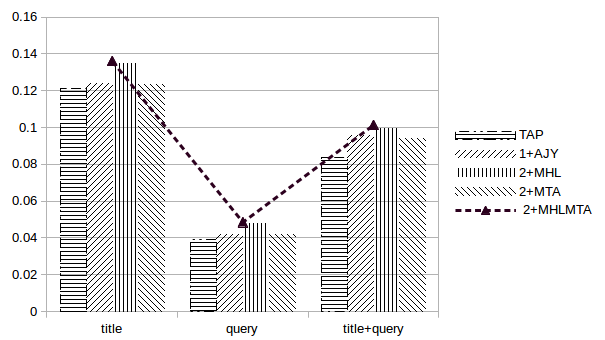
\includegraphics[height=4.05cm, width=0.520\textwidth]{map_measurements.png}
    \vspace{-0.75cm}
    \caption{Graphical comparison of the MAP measurement for the 5 different indexing schemes and the 3 different query parsing techniques}
    \label{fig:map}
\end{figure}
\vspace{-0.05cm}


%=================================================
\begin{figure}[H]
    \centering 
 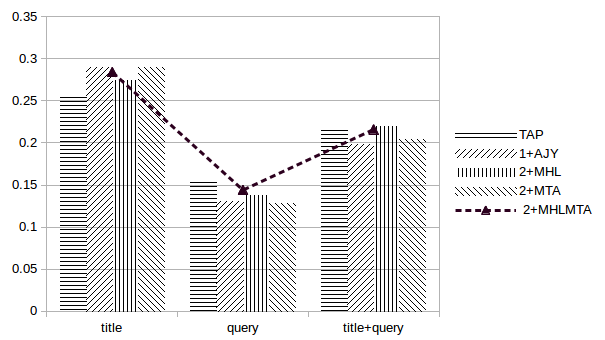
\includegraphics[height=4.05cm,width=0.520\textwidth]{precision_after_10.png}
 \vspace{-0.75cm}
    \caption{Graphical comparison of the precision after 10 documents retrieved for the 5 different indexing schemes and the 3 different query parsing techniques}
    \label{fig:p_10}
\end{figure}
\vspace{-0.5cm}
%=================================================
\begin{figure}[H]
    \centering 
  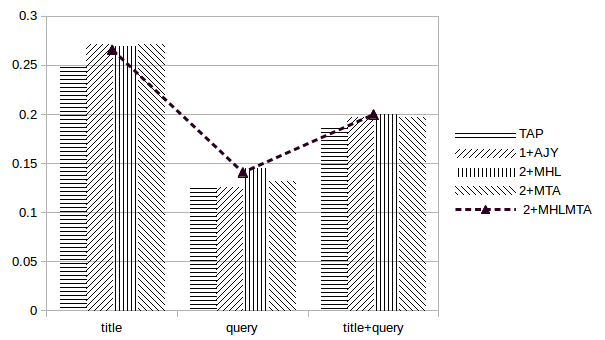
\includegraphics[height=4.05cm,width=0.520\textwidth]{precision_after_20.png}
    \vspace{-0.75cm}
    \caption{Graphical comparison of the precision after 20 documents retrieved measurement for the 5 different indexing schemes and the 3 different query parsing techniques}
    \label{fig:p_20}
\end{figure}
\vspace{-0.5cm}
%=================================================
\begin{figure}[H]
    \centering 
  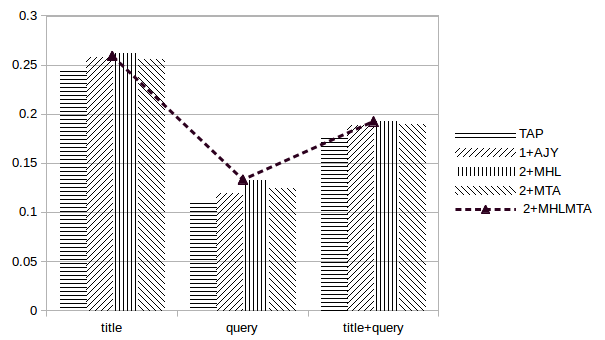
\includegraphics[height=4.05cm,width=0.520\textwidth]{precision_after_30.png}
  \vspace{-0.75cm}
    \caption{Graphical comparison of the precision after 30 documents retrieved measurement for the 5 different indexing schemes and the 3 different query parsing techniques}
    \label{fig:p_30}
\end{figure}
\vspace{-0.5cm}
%=================================================
\begin{figure}[H]
    \centering 
  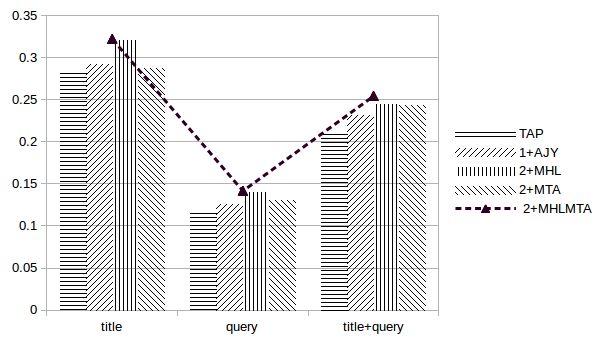
\includegraphics[height=4.05cm,width=0.520\textwidth]{interpolated_R_P_at_10.png}
  \vspace{-0.75cm}
    \caption{Graphical comparison of the IRPA at 0.10 recall, for the 5 different indexing schemes and the 3 different query parsing techniques}
    \label{fig:irp_at_10}
\end{figure}
\vspace{-0.5cm}
%=================================================
\begin{figure}[H]
    \centering 
  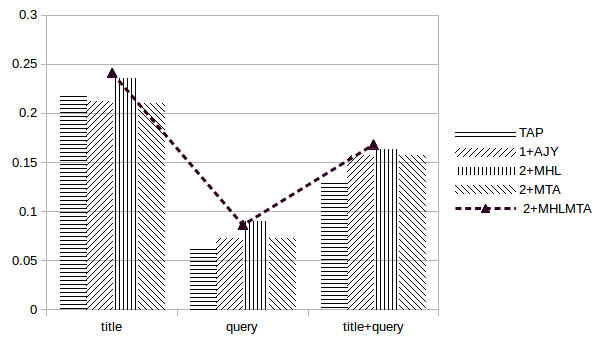
\includegraphics[height=4.05cm,width=0.520\textwidth]{interpolated_R_P_at_20.png}
  \vspace{-0.75cm}
    \caption{Graphical comparison of the IRPA at 0.20 recall, for the 5 different indexing schemes and the 3 different query parsing techniques}
    \label{fig:irp_at_20}
\end{figure}
\vspace{-0.3cm}
%=================================================
We notice from the MAP measurements that the $5^{th}$ indexing scheme performs the best in all 3 query parsing scenarios. Respectively, we observe that the 'title' topic-parsing technique A accomplishes the best MAP performance with all 5 indexing scheme scenarios. Furthermore, we notice from the Precision after 10, 20 and 30 documents retrieved, that there is no dominant indexing methodology. Moreover, we notice that the performance of the 2nd and 4th indexing methodology is very similar in almost every query parsing and number of retrieved documents scenario. We also notice that the precision after 10, 20 and 30  documents retrieved is higher when the 'title' parsing technique A is utilised instead of the other 2 initial query extraction techniques. Additionally, we recognise that the measurements of the IRPA at 0.10 and 0.30 recall is always higher when using the $5^{th}$ indexing scheme. The same can also be said for the IRPA at 0.20 recall, but in this case there is a small exception when utilising the 'query' topic-parsing technique, where we observed that the $5^{th}$ indexing scheme accomplishes the best score after the $3^{rd}$ indexing method. Finally, we observed that the IRPA at 0.10, 0.20 and 0.30 recall is always higher when using the 'title' topic-parsing technique.  

\vspace{-0.3cm}
\begin{figure}[H]
    \centering 
  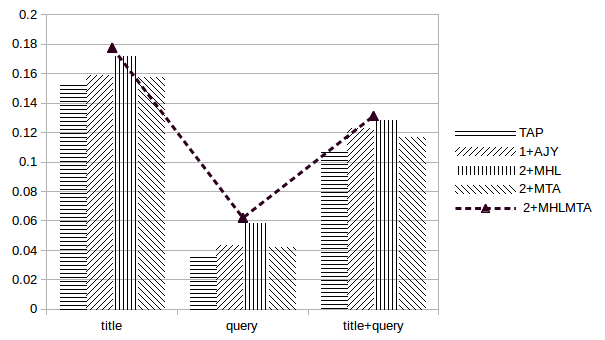
\includegraphics[height=4.05cm,width=0.520\textwidth]{interpolated_R_P_at_30.png}
  \vspace{-0.75cm}
    \caption{Graphical comparison of the IRPA at 0.30 recall, for the 5 different indexing schemes and the 3 different query parsing techniques}
    \label{fig:irp_at_30}
\end{figure}
%=================================================
\vspace{-0.6cm}
%=================================================
\section{Conclusion}

We focused on discovering how alternative indexing schemata affect performance and how different extraction techniques of the initial query from CLEF topics affect performance. We found out that the IR performance is improved substantially when using the $5^{th}$ indexing scheme, which enables us to draw the conclusion that adding more fields to the PubMed  indexer is actually a positive contributor for the retrieval  effectiveness of an IR system such as L4IR. We look forward to increase the number of our experiments using the L4IR system, to index additional fields of the PubMed documents and to find methodologies for indexing and query parsing new empirical test collections. Finally we also plan to test more retrieval models that are available in the L4IR system and make use of Active Learning to enhance the ranking by using feedback from reviewers. 
%=================================================

%\end{document}  % This is where a 'short' article might terminate

\appendix

% Appendix A
\section{Appendix}
We have included a README.md file which contains guide instructions, 2 iPython Notebooks with the code for the automation of our experiments, a Python script for parsing the topics to produce queries, 5 different Java classes one for each indexing methodology and the updated 'IndexerApp' Java class of L4IR.



\bibliographystyle{ACM-Reference-Format}
\bibliography{sample-bibliography} 

\end{document}
